\chapter{MARG Sensors}
\label{ch:MARG}

Broadly speaking, sensors are physical devices used to detect changes in the output of a system. MARG sensors is a collective term for magnetic, angular rate, and gravitational sensors, which encompasses inertial sensors, as well as magnetic field sensors, also referred to as magnetometers. Inertial sensors itself generally fall into two categories: instruments sensing linear inertial displacement (accelerometers) and rotational inertial rate sensors (gyroscopes). They are applied in various contexts to quantify vibration, motion, and shock \cite{bhattacharyya_inertial_sensors_applications_13}. Particularly, the development of \gls{MEMS} opened up many medical applications as stated in Section \ref{sec:MARG_sensors_medical}. They have low manufacturing costs, small physical size, and low power consumption \cite{bhattacharyya_inertial_sensors_applications_13}. This chapter compiles the functional principles of MARG sensors and introduces \glspl{IMU} as a combination of those. At the end of the chapter the aforementioned GaitWatch device that was used to gather the movement data for the experiments is described in detail.

\section{Accelerometers}

Accelerometers measure the acceleration of an object relative to an inertial frame. Since acceleration cannot be sensed directly, the force exerted on a reference mass is measured. The resultant acceleration is computed according to Newton's second law $\mathbf{f} = m \cdot \mathbf{a}$, where $ \mathbf{f} \in \mathbb{R}^3$ denotes the force vector, $m$ the mass, and $\mathbf{a} \in \mathbb{R}^3$ the acceleration vector. Usually, an accelerometer consists of a small proof mass connected via a spring to the case of the instrument. The proof mass is displaced  by $\Delta x$ with respect to the case, when the instrument experiences a certain acceleration along its sensitive axis. Disregarding drag force, the displacement is directly proportional to the force exerted by the mass and thus to the acceleration. Therefore, by measuring the displacement of the proof mass the acceleration can be obtained. Figure \ref{fig:accelerometer} shows the displacement $\Delta x$ of the mass in respect to the case of the instrument for three different conditions: (a) at rest or in uniform motion, (b) accelerating, and (c) at rest, being exposed to the gravity $g$. According to how the mass displacement is sensed, accelerometers can be classified as resistive, capacitive, and piezoelectric. Besides, there are surface acoustic wave, fibre optic, vibrating beam and solid-state \gls{MEMS} accelerometers. To obtain a three-dimensional accelerometer, three single-axis accelerometers are mounted together. Although a mutually orthogonal mount is common practice, any non-coplanar arrangement is acceptable, as long as the angles between the sensitive axes are known. Nowadays most accelerometers are manufactured using MEMS technology, which was developed for the military and aerospace markets in the 1970s \cite{bhattacharyya_inertial_sensors_applications_13}. 

\begin{figure}
\centering
\begin{tikzpicture}[scale=0.95, auto, thick, node distance=3cm,>=latex']
    \pgftext{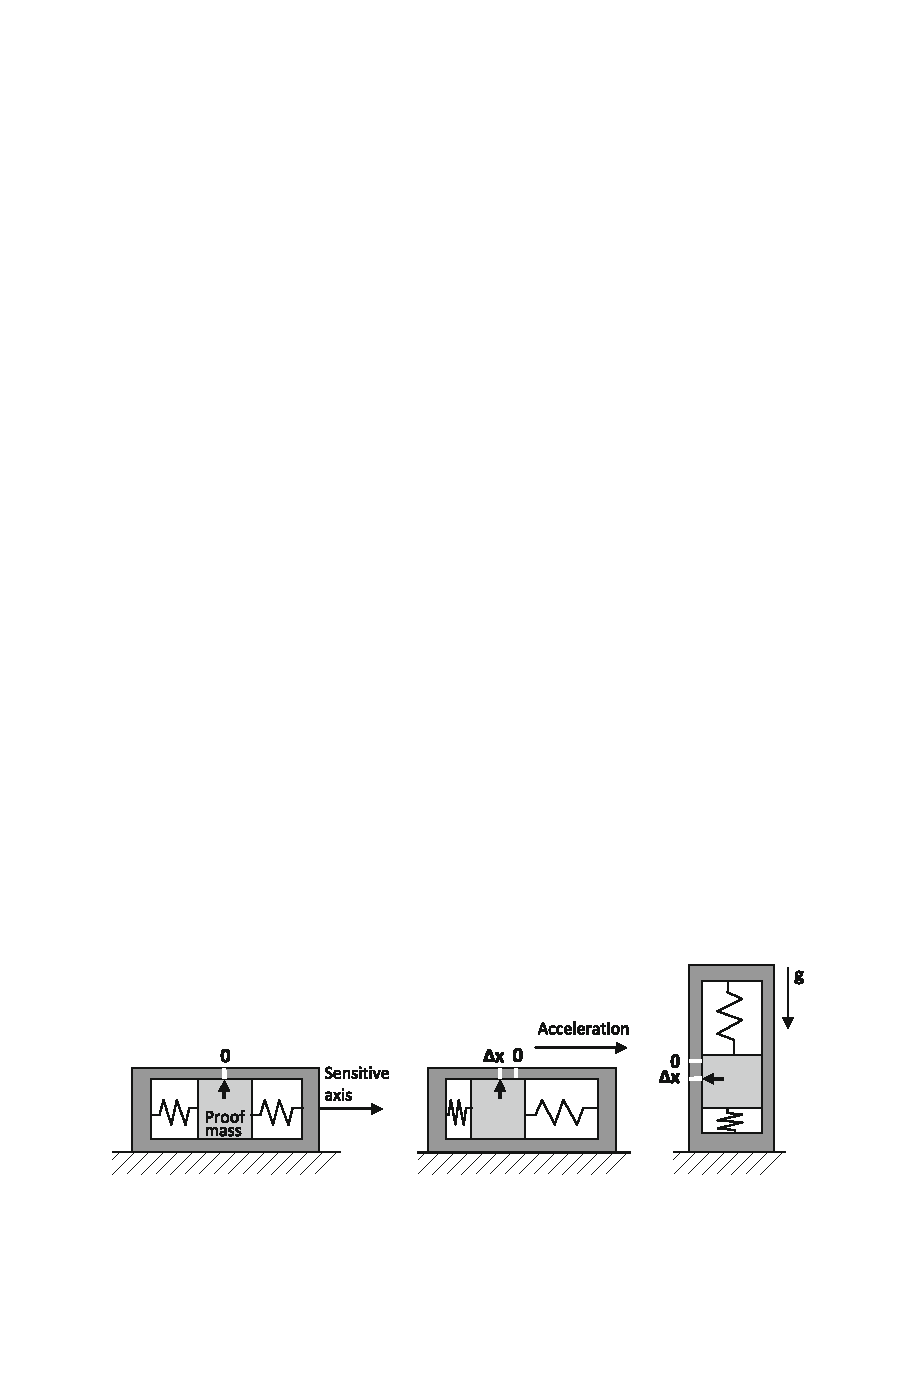
\includegraphics[width=13.5cm]{images/accelerometer}} at (0pt,0pt);
    \node [] (a) at (-6.7, -1.1) {(a)};
    \node [] (b) at (-1.1, -1.1) {(b)};
    \node [] (c) at (3.9, -1.1) {(c)};
    \node [] (c) at (-4.525, 0.44) {$0$};
    \node [] (c) at (1.03, 0.44) {$0$};
    \node [] (c) at (4, 0.26) {$0$};
    \node [] (c) at (0.58, 0.44) {$\Delta x$};
    \node [] (c) at (3.82, -0.08) {$\Delta x$};
    \node [] (c) at (6.5, 1.5) {$\mathbf{g}$};
    \node [] (c) at (-4.525, -0.75) {\scriptsize Proof};
    \node [] (c) at (-4.525, -1.05) {\scriptsize mass};
    \node [] (c) at (-2, -0.05) {\scriptsize Sensitive};
    \node [] (c) at (-2, -0.45) {\scriptsize axis};
    \node [] (c) at (2.2, 0.85) {\scriptsize Acceleration};
\end{tikzpicture}
\caption{A mass-and-spring accelerometer under different conditions: (a) at rest or in uniform motion, (b) accelerating, and (c) at rest, being exposed to the gravity $\mathbf{g}$, from \cite{bhattacharyya_inertial_sensors_applications_13}.}
	\label{fig:accelerometer}
\end{figure}


\section{Gyroscopes}

Gyroscopes are used for measuring and maintaining angular orientation. In essence, based on two different physical principles, namely the Sagnac and Coriolis effect, gyroscopes sense angular velocity, which is why they are also referred to as angular velocity sensors or angular rate sensors. By integrating the angular velocity the rotation angle can obtained. Here we will only elaborate on the working principle of vibrating gyroscopes, since they are utilised in the GaitWatch device. \citeauthor{armenise2010advances} give a comprehensive overview of current gyroscope technologies in \cite{armenise2010advances}.

Coriolis vibratory gyroscopes, or vibrating gyros for short, sense angular velocity based on the effect of Coriolis force on a vibrating mass. The Coriolis force is a fictitious force experienced by a mass $m$ moving in a rotating reference frame. It can be calculated as: $\mathbf{f}_C = -2m(\bm{\omega} \times \mathbf{v})$, where $\mathbf{v}$ is the mass velocity in the rotating reference frame and $\bm{\omega}$ is the angular velocity of the reference frame. As seen in this equation the Coriolis force is only present when the mass varies its distance with respect to the spin axis. Otherwise, if $\bm{\omega}$ and $\mathbf{v}$ are parallel, the cross product becomes zero. The two degree-of-freedom spring-mass-damper system shown in Figure \ref{fig:gyroscope} serves as a simple model of a vibrating angular rate sensor. The mass $m$ can move along the $x$ and $y$-axis, respectively. The angular velocity around the $z$-axis is denoted with $\omega$. The drive or primary oscillating mode, that is, the oscillation along $x$, is excited by the force $F_x$ directed along the $x$-axis. The oscillation along $y$, called sense or secondary oscillating mode, is due to system rotation around the $z$-axis. $D_x$ and $D_y$ are the damping coefficients and $k_x$ and $k_y$ are the spring constants along the $x$ and $y$-axis, respectively. Typically, the primary oscillating mode is excited by a sinusoidal force with an angular frequency close to the resonance frequency, so that $\Omega_x \cong \sqrt{k_x/m}$. Its amplitude is kept constant at $a_x$. As shown in \cite{armenise2010advances},the amplitude of the sense mode is then given by

\begin{equation}
  a_y = -\frac{2 a_x \Omega_x \omega}{\sqrt{(\Omega^2_x - \Omega^2_y)^2 + \Omega^2_x \Omega^2_y / Q^2_y}}\,,
\end{equation}

\noindent
where $\Omega_y=\sqrt{k_y/m}$ is the resonance frequency of the secondary resonator and $Q_y = \sqrt{m k_y}/D_y$ its quality factor. The amplitude $a_y$ is directly proportional to the angular rate of the two degree-of-freedom spring-mass-damper system. Thus, $\omega$ can be estimated by measuring the amplitude of the oscillation along the $y$-axis.

Usually, vibrating gyroscopes are manufactured using MEMS technology. MEMS gyros are of low to medium accuracy \cite{bhattacharyya_inertial_sensors_applications_13}, but due to their size they are ideally suited for medical applications.

\begin{figure}
\centering
\begin{tikzpicture}[auto, thick,>=latex', cross/.style={path picture={ 
  \draw[black]
(path picture bounding box.south east) -- (path picture bounding box.north west) (path picture bounding box.south west) -- (path picture bounding box.north east); }}]

\tikzstyle{spring}=[thick,decorate,decoration={zigzag,pre length=0.3cm,post length=0.3cm,segment length=6}]
\tikzstyle{damper}=[thick,decoration={markings,  
  mark connection node=dmp,
  mark=at position 0.5 with 
  {
    \node (dmp) [thick,inner sep=0pt,transform shape,rotate=-90,minimum width=8pt,minimum height=7pt,draw=none] {};
    \draw [thick] ($(dmp.north east)+(4pt,0)$) -- (dmp.south east) -- (dmp.south west) -- ($(dmp.north west)+(4pt,0)$);
    \draw [thick] ($(dmp.north)+(0,-4pt)$) -- ($(dmp.north)+(0,4pt)$);
  }}, decorate]
\tikzstyle{ground}=[fill,pattern=north east lines,draw=none,minimum width=0.75cm,minimum height=0.3cm]


\node (M) [draw, minimum width=3cm, minimum height=3cm] {};

\node (ground) [ground,anchor=north,yshift=-1.5cm,minimum width=3.5cm] at (M.south) {};
\draw (ground.north east) -- (ground.north west);

\node (wall) [ground, rotate=-90, minimum width=3.5cm,yshift=-3cm] {};
\draw (wall.north east) -- (wall.north west);

\draw [spring] (wall.170) -- node [label={[label distance=-0.2cm]above:$k_x$}] {}($(M.north west)!(wall.170)!(M.south west)$);
\draw [damper] (wall.10) -- node [label={[label distance=-0.1cm]above:$D_x$}] {}($(M.north west)!(wall.10)!(M.south west)$);

\draw [spring] (ground.170) -- node [label={[label distance=0.09cm]right:$k_y$}] {}($(M.south east)!(ground.170)!(M.south west)$);
\draw [damper] (ground.10) -- node [label={[label distance=0.08cm]right:$D_y$}] {}($(M.south east)!(ground.10)!(M.south west)$);      

    \node[coordinate] (X) at (5,-1) {};
    \node[coordinate] (Y) at (3,1) {};
    \node[coordinate] (O) at (3, -1) {};
    
    \draw[->] (O) -- node[name=x] {$x$}(X);
    \draw[->] (O) -- node[name=y] {$y$}(Y);
    \node [draw,circle, fill=white,cross,minimum width=0.15 cm, label={[anchor=south west]below:$z$}](z) at (3, -1){};
    
    \draw[-stealth] (0.15,1) arc (80:390:1);
    
    \node at (0.6, 0.8) (angle1) {$\omega$};
    \node at (-1.05, 1.1) (angle1) {$m$};
    
    \draw [-stealth, align=center] (-0.5,2) -- node[name=Fx] {$F_x$} (0.5,2);

    
\end{tikzpicture}
\caption{A simple model of a Coriolis vibratory gyroscope: Two degree-of-freedom spring-mass-damper system in a rotating reference frame, from \cite{armenise2010advances}.} \label{fig:gyroscope}
\end{figure} 
 

\section{Magnetometers}

Magnetometers measure the strength and the direction of the magnetic field at a point in space. There are numerous techniques used to produce magnetic field sensors, which exploit a broad range of physical phenomena \cite{lenz_magnetic_2006}. \citeauthor{lenz_magnetic_2006} give a complete survey of common technologies used for magnetic field sensing in \cite{lenz_magnetic_2006}. Many \gls{MEMS} magnetometers sense mechanical motion of a MEMS structure due to Lorentz force and estimate the strength of the magnetic field according to the displacement. When an external magnetic field interacts with a current-carrying silicon MEMS structure the Lorentz force causes a displacement of this structure. Piezoresistive, capacitive, or optical sensing can be used to detect the displacement of the MEMS structure. MEMS Lorentz force magnetometers are free from hysteresis, require no specialised materials and can be monolithically integrated with other MEMS inertial sensors \cite{thompson_lorentz_2011}.

\section{Inertial Measurement Units}

Devices using a combination of accelerometers and gyroscopes to measure the orientation of a rigid body with up to six degrees of freedom are referred to as \glspl{IMU}. If they include additional magnetometers they are termed \glspl{MIMU}. The number of degrees of freedom states the number of independent motions, with respect to a reference frame, that are allowed to the body in space. \glspl{MIMU} are portable and relatively inexpensive. They can be easily attached to the body and thus allow non-clinical longterm application. Their drawbacks are complex calibration procedures and drift behaviour over time, depending on intensity and duration of the measurement interval. Hence, in order to maintain a satisfactory degree of precision, periodical recomputation of the calibration parameters is required \cite{olivares_vicente_signal_2013}.

\subsection{The GaitWatch}

The above-mentioned GaitWatch device was designed to monitor the motion of patients while attached to the body. It was developed at the Department of Neurology of the Ludwig-Maximilians University in Munich, Germany, in association with the Department of Signal Theory, Telematics and Communications of the University of Granada, Spain. The system is composed of a set of embedded magnetic and inertial sensors wired to a box containing a microcontroller. This microcontroller is in charge of collecting data from the embedded box sensors, as well as from the external measurement units, and storing them on a memory card. The various units are placed at the patient's trunk, arms, thighs, and shanks as shown in Figure \ref{fig:GaitWatch_placement}. The components of the three different kinds of subunits are described below:

\begin{itemize}

\item \textsc{type a -- thighs and shanks:} 

IMU Analog Combo Board with 5 Degrees of Freedom \cite{IMU5}, containing an IDG500 biaxial gyroscope, from which only y-axis is actually used, with a measurement range of ±500\,°/s \cite{IDG500} and a ±3\,g triaxial accelerometer, ADXL335 \cite{ADXL335}.

\item \textsc{type b -- arms:}

IDG500 biaxial gyroscope with a measurement range of ±500\,°/s \cite{IDG500}.

\item \textsc{type c -- trunk:}

ADXL345 triaxial accelerometer with a programmable measurement range of ±2/±4/±8/±16\,g \cite{ADXL345},
IMU3000 triaxial gyroscope with a programmable measurement range of ±250/±500/±1000/±3000°/s \cite{IMU3000}, 
Micromag3 \allowbreak triaxial magnetometer with a measurement range of ±11\,Gauss \cite{MicroMag3}, AL-XAVRB board containing an AVR ATxmega processor \cite{AVRATxmega}.

\end{itemize}

\begin{figure}
\centering
\begin{tikzpicture}[scale=0.95, auto, thick, node distance=3cm,>=latex']
    \pgftext{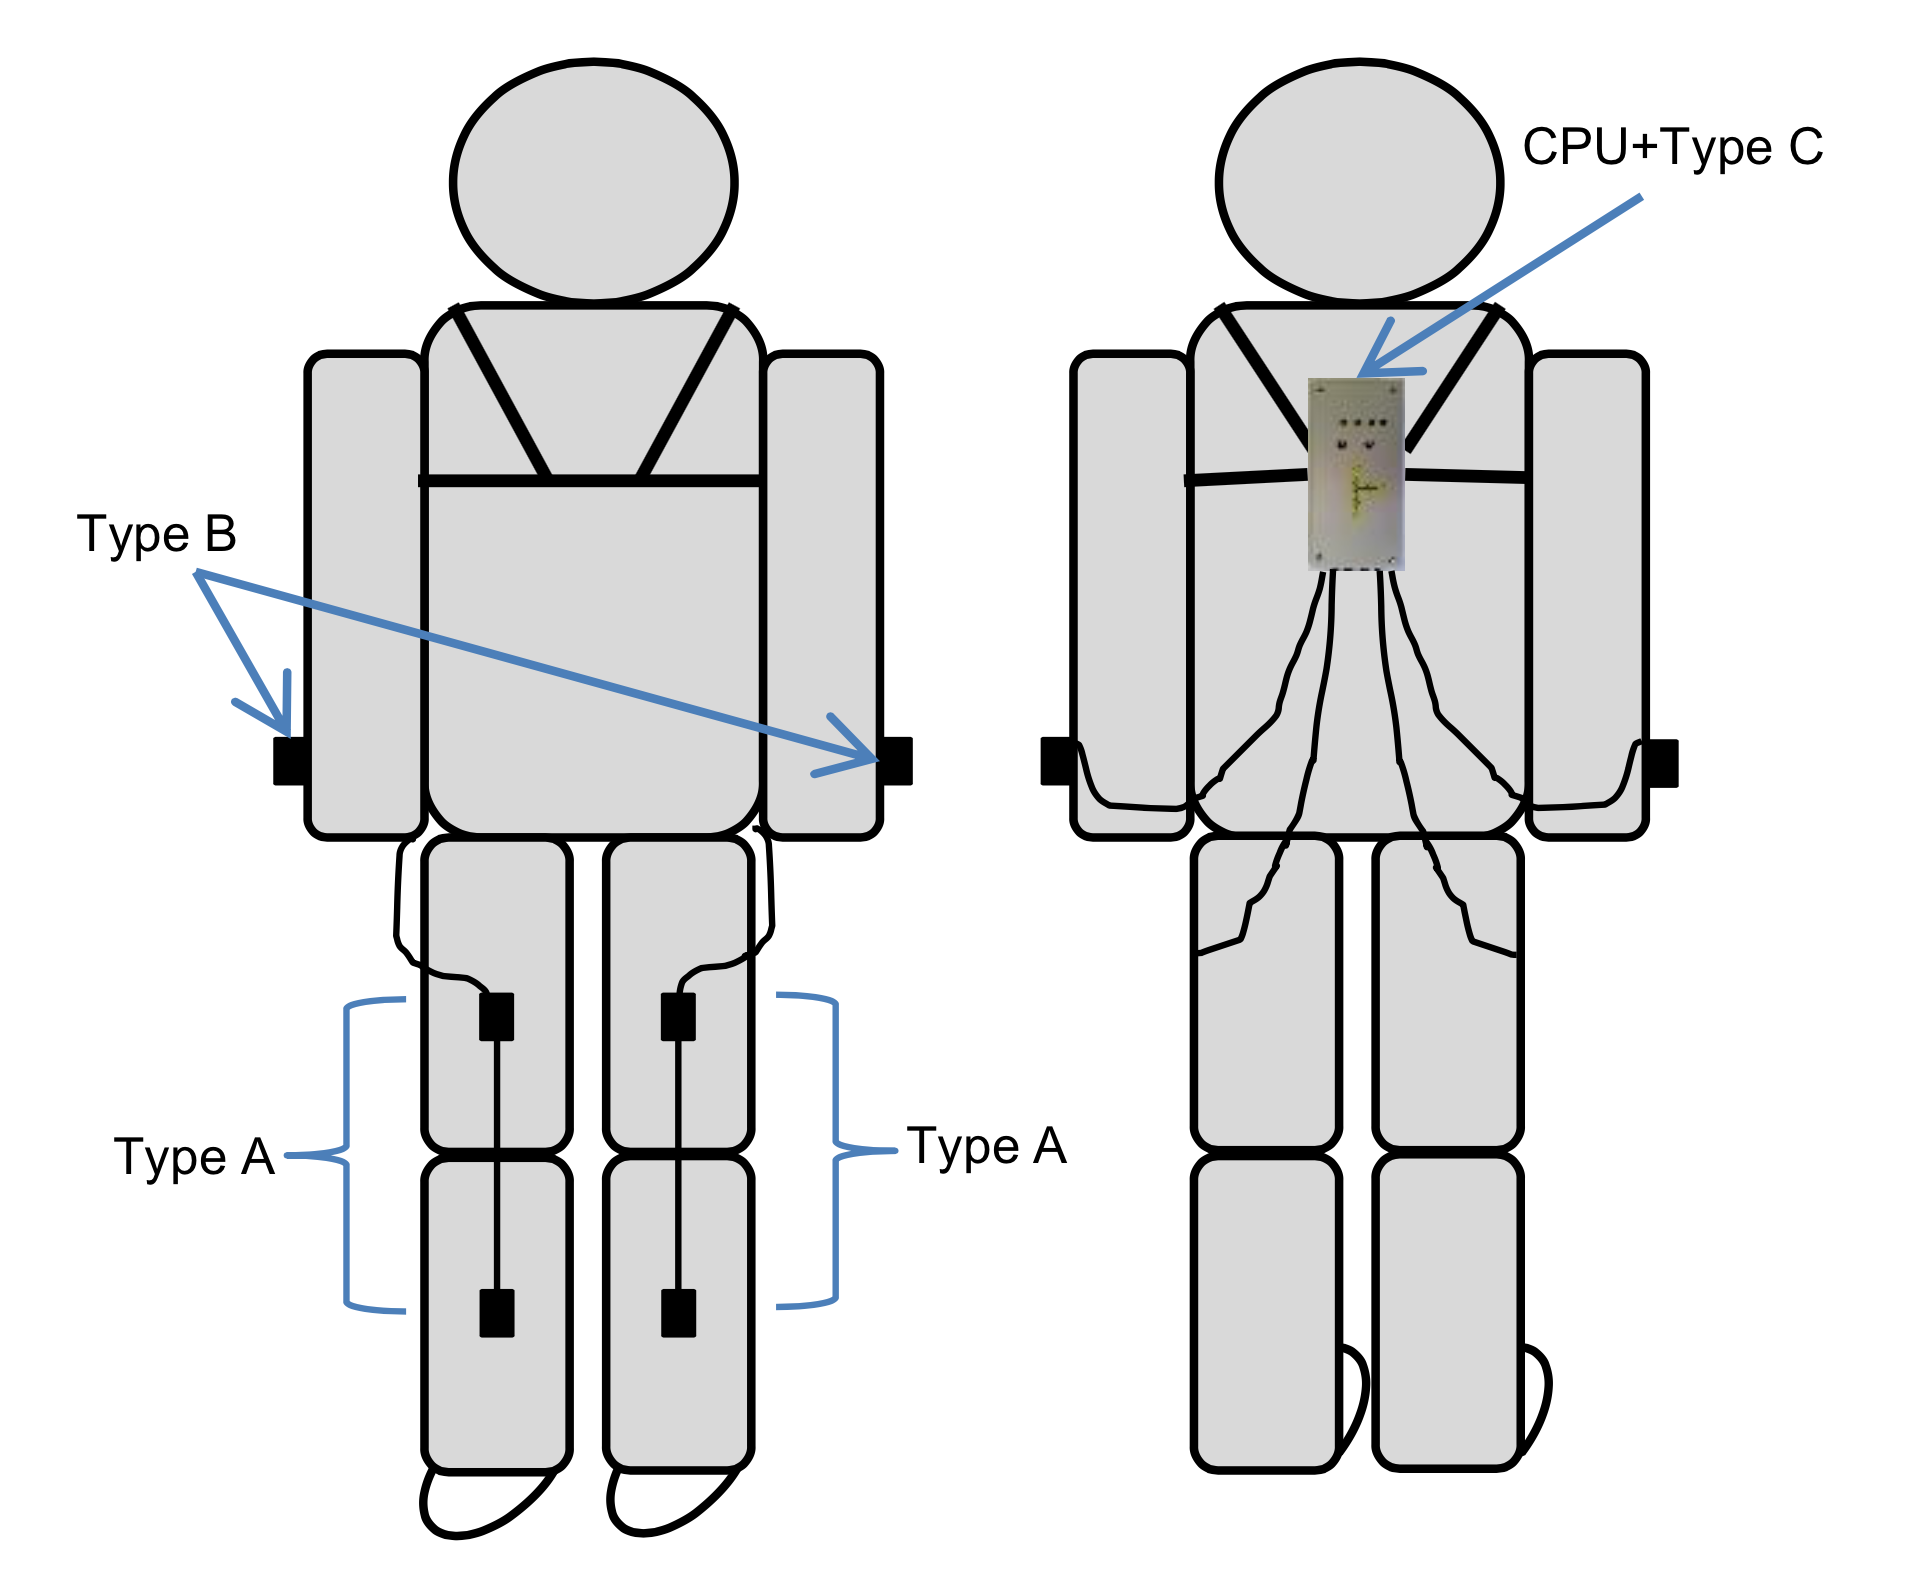
\includegraphics[width=10cm]{images/GaitWatch_placement}} at (0pt,0pt);
    \node [] (a) at (-4.4, -2) {Type A};
    \node [] (b) at (-4.5, 0.1) {Type B};
    \node [] (c) at (4.45, 3.25) {Type C};
\end{tikzpicture}
\caption{Placement of the GaitWatch components at the body, from \cite{olivares_vicente_gaitwatch_2013}.}
	\label{fig:GaitWatch_placement}
\end{figure}





